\documentclass[a4paper,11pt]{article}

\usepackage[utf8]{inputenc}
\usepackage{graphicx}
\usepackage{caption}
\usepackage{subcaption}
\usepackage{float}
\usepackage{amsmath}
\usepackage{pgfplots}
\usepackage{ffcode}
\usepackage{booktabs}
\usepackage{listings}
\usepackage{xcolor}
\usepackage{listings}
\usepackage{array}
\usepackage{tikz}
\usepackage{algorithm}
\usepackage{algpseudocode}
\usetikzlibrary{calc,patterns,angles,quotes}

\pgfplotsset{compat=1.18} 

\begin{document}
	
\title{
	\textbf{Quadson}
}
\author{Ying Pei Lin}
\date{Spring 2025}
\maketitle

\section*{Introduction}

Quadson is a 3D printed quadruped robot designed as a platform for exploring advanced robotic motion and control.
This document includes its forward kinematics, inverse kinematics, differential kinematics and expands to body kinematics.
Following this analysis, we will introduce the process of performing simultion in Pybullet and using deep
reinforcement learning to improve the robot's control and performance.

\section*{Forward Kinematics}

For each leg of the robot, we define the reference frame with its origin at point $p_1$. 
Two motors are positioned at $p_1$ and $p_5$ respectively, and the third motor
connected to the entire leg assembly, controls the rotation around x axis. The remaining joints in the leg are all passive.

\begin{center}
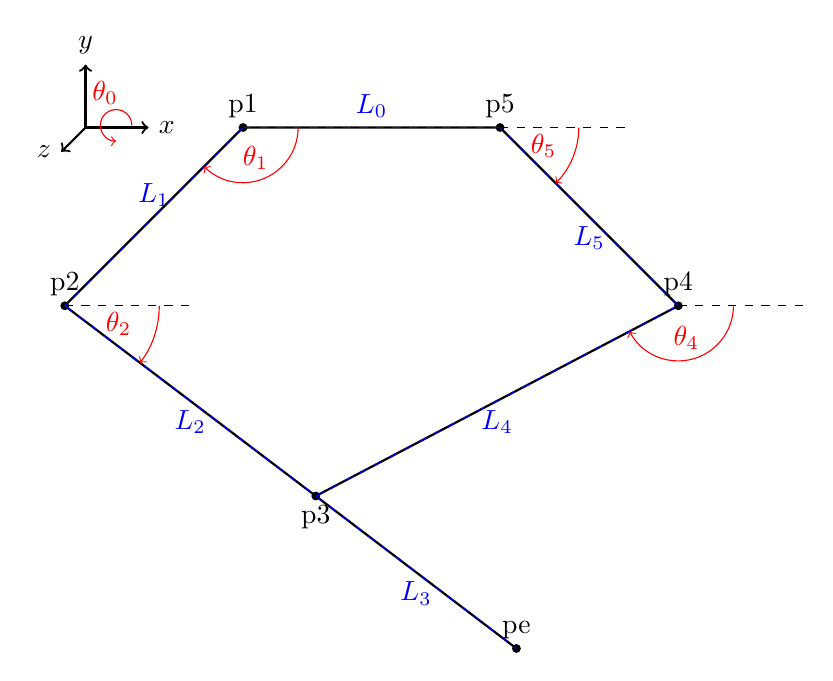
\begin{tikzpicture}[scale=0.4]
	% Points
	\coordinate (p1) at (0,0);
	\coordinate (p2) at (-5.66,-5.66);
	\coordinate (p2_hori) at (-1.66,-5.66);
	\coordinate (p3) at (2.31,-11.70);
	\coordinate (pe) at (8.68,-16.54);
	\coordinate (p4) at (13.82,-5.66);
	\coordinate (p4_hori) at (17.82,-5.66);
	\coordinate (p5) at (8.16,0);
	\coordinate (p5_hori) at (12.16,0);

	% Lines
	\draw[thick] (p1) -- (p2) -- (p3) -- (p4) -- (p5) -- (p1);
	\draw[thick] (p3) -- (pe);
	\draw[dashed] (p2) -- (p2_hori);
	\draw[dashed] (p4) -- (p4_hori);
	\draw[dashed] (p5) -- (p5_hori);
	
	% Axis
	\draw[thick,->] (-5,0,0) -- (-3,0,0) node[right] {$x$};
	\draw[thick,->] (-5,0,0) -- (-5,2,0) node[above] {$y$};
	\draw[thick,->] (-5,0,0) -- (-5,0,2) node[left] {$z$};
	\draw[red,->] (-3.8,-0.2,-0.7) arc[start angle=0,end angle=270,radius=0.5cm] node[midway,above] {$\theta_0$};

	% Point tags
	\foreach \p in {p1, p2, pe, p4, p5} {
			\fill[black] (\p) circle (4pt);
			\node[above] at (\p) {\p};
	}
	\fill[black] (p3) circle (4pt);
	\node[below] at (p3) {p3};

	% Length tags
	\draw[blue, dashed] (p1) -- (p5) node[midway, above] {$L_{0}$};
	\draw[blue, dashed] (p1) -- (p2) node[midway, above] {$L_{1}$};
	\draw[blue, dashed] (p2) -- (p3) node[midway, below] {$L_{2}$};
	\draw[blue, dashed] (p3) -- (pe) node[midway, below] {$L_{3}$};
	\draw[blue, dashed] (p3) -- (p4) node[midway, below] {$L_{4}$};
	\draw[blue, dashed] (p4) -- (p5) node[midway, below] {$L_{5}$};

	% Angle tags
	\pic [draw=red, text=red, <-, "$\theta_1$", angle radius=0.7cm] {angle=p2--p1--p5};
	\pic [draw=red, text=red, <-, "$\theta_2$", angle radius=1.2cm] {angle=p3--p2--p2_hori};
	\pic [draw=red, text=red, <-, "$\theta_4$", angle radius=0.7cm] {angle=p3--p4--p4_hori};
	\pic [draw=red, text=red, <-, "$\theta_5$", angle radius=1cm] {angle=p4--p5--p5_hori};
\end{tikzpicture}
\end{center}

The following algorithm takes the angle of three motors as input and computes the position of the end effector.
The process incorporates several safety check, prevent configurations that could potentially damage the mechanism.

\begin{algorithm}[H]
	\caption{Compute Leg End-Point}
	\begin{algorithmic}[1]
			\Require Motor angles $\theta_0, \theta_1, \theta_5$
			\State Perform safety checks and limit angles
			\State Compute initial 2D joint positions:
			\[
				p_2 = (L_1 \cos \theta_1, -L_1 \sin \theta_1), \quad
				p_5 = (L_0, 0), \quad
				p_4 = p_5 + (L_5 \cos \theta_5, -L_5 \sin \theta_5)
			\]
			\State Compute distances:
			\[
					L_{14} = \| p_4 - p_1 \|, \quad
					L_{24} = \| p_4 - p_2 \|
			\]
			\If{$L_{24} < 5$ or $L_{24} > L_2 + L_4$}
					\State Mark as unsafe and return previous endpoint
			\EndIf
			\State Solve for $p_3$ using angles:
			\[
					\theta_2 = \cos^{-1} \left( \frac{L_2^2 + L_{24}^2 - L_4^2}{2 L_2 L_{24}} \right) +
										 \cos^{-1} \left( \frac{L_1^2 + L_{24}^2 - L_{14}^2}{2 L_1 L_{24}} \right) - (\pi - \theta_1)
			\]
			\[
					p_3 = p_2 + L_2 (\cos \theta_2, -\sin \theta_2)
			\]
			\State Compute endpoint:
			\[
					p_e = p_2 + (L_2 + L_3)(\cos \theta_2, -\sin \theta_2)
			\]
			\State Transform to 3D using rotation matrix:
			\[
					R_{\theta_0} =
					\begin{bmatrix}
							1 & 0 & 0 \\
							0 & \cos(-\theta_0) & -\sin(-\theta_0) \\
							0 & \sin(-\theta_0) & \cos(-\theta_0)
					\end{bmatrix}
			\]
			\State Update joint angles and return $p_e$
	\end{algorithmic}
\end{algorithm}

\section*{Inverse Kinematics}

In real world scenarios, controlling position of the end effector to reach to a certain position
is often more pratical than setting the angles directly. For example, to move the end effector along 
a defined trajectory, achieving this by manually adjusting the three motor angles is nearly impossible 
due to the complexity and interdependence of the joint movements. 

Therefore we need the following algorithm 
to compute the angles of the motor corresponding to a given target position.

\begin{algorithm}[H]
	\caption{Compute Joint Angles from End-Point}
	\begin{algorithmic}[1]
			\Require End-point position $(x, y, z)$
			\State Calculate angle of motor 0:
			\[
				\theta_0 = -\tan^{-1} \left( \frac{z}{-y} \right)
			\]
			\State Translate points from 3D to 2D using rotation matrix:
			\[
				R_{\theta_0} =
					\begin{bmatrix}
							1 & 0 & 0 \\
							0 & \cos(-\theta_0) & -\sin(-\theta_0) \\
							0 & \sin(-\theta_0) & \cos(-\theta_0)
					\end{bmatrix}
			\]
			\[
				\begin{bmatrix} x' \\ y' \\ z' \end{bmatrix} = \text{transformation matrix} \times \begin{bmatrix} x \\ y \\ z \end{bmatrix}
			\]
			\State Calculate angle 1:
			\[
					L_{1e} = \| (x', y') \|, \quad
					\theta_{e15} = \tan^{-1} \left( \frac{-y'}{x'} \right)
			\]
			\[
					\theta_{e12} = \cos^{-1} \left( \frac{L_1^2 + L_{1e}^2 - (L_2 + L_3)^2}{2 L_1 L_{1e}} \right)
			\]
			\[
					\theta_1 = \theta_{e15} + \theta_{e12}
			\]
			\State Compute positions of joints:
			\[
					p_1 = (0, 0), \quad
					p_2 = (L_1 \cos \theta_1, -L_1 \sin \theta_1)
			\]
			\[
					p_3 = \frac{(pe_2d \cdot L_2) + (p_2 \cdot L_3)}{L_2 + L_3}, \quad
					p_5 = (L_0, 0)
			\]
			\State Calculate angle 5:
			\[
				\theta_{350} = \tan^{-1} \left( \frac{-p_3[1]}{L_0 - p_3[0]} \right)
			\]
			\[
					\theta_{354} = \cos^{-1} \left( \frac{L_{35}^2 + L_5^2 - L_4^2}{2 L_{35} L_5} \right), \quad
					L_{35} = \| p_3 - p_5 \|
			\]
			\[
					\theta_5 = \pi - (\theta_{350} + \theta_{354})
			\]
			\State Perform safety checks on angles:
			\State \Return $(\theta_0, \theta_1, \theta_5)$
	\end{algorithmic}
\end{algorithm}

\section*{Differential Kinematics}

\section*{Body Kinematics}

\section*{Movement Control}

\section*{Simulation}

\section*{Deep Reinforcement Learning}

\section*{Conclusion}

\end{document}